\section{问题表述与双时间尺度决策建模}
\subsection{共同目标与可行决策}
仅在任务完成时给予反馈，会使较长时间未完成的任务迟迟无法影响即时奖励。尤其当不同类别的完成率明显不同时，完成样本的平均时延还可能因样本选择而下降。为使所有仍在系统内的任务持续参与评价，令$\mathcal U_m$表示物理步$m$服务结束后尚未完成的父任务集合，$w_p$为$p$类任务的无量纲权重。一个物理步的加权驻留量为
\begin{equation}
 H[m]=\delta\sum_{\nu\in\mathcal U_m}w_{p_\nu}.
 \label{eq:holding}
\end{equation}
$H[m]$以task\,s计，其中任务数视为计数单位，采用$w_{\mathrm H}=10$、$w_{\mathrm L}=1$。该集合同时包括上传、待拆分、转发和计算阶段的父任务。无论父任务生成多少分片，其驻留权重只计一次，避免“拆得越多、惩罚越大”的计数偏差。

驻留代价与完成时延存在联系，但二者不能在有限窗口中直接混同。设连续时间$u$处的加权未完成任务数为$N_w(u)$，观察终点为$T$，且初始系统为空，则理想连续记账满足
\begin{equation}
 \begin{aligned}
 &\int_0^T N_w(u)\,\dd u\\
 &\quad=\sum_{\nu:\tau_\nu^{\mathrm b}<T}
 w_{p_\nu}\big[\min\{\tau_\nu^{\mathrm f},T\}-\tau_\nu^{\mathrm b}\big].
 \end{aligned}
 \label{eq:holdingidentity}
\end{equation}
其中，$\tau_\nu^{\mathrm f}$为父任务完成时刻，未完成时取$+\infty$。右侧既包含已完成任务的完整驻留，也包含未完成任务截至$T$已经经历的等待。式\eqref{eq:holding}采用步末离散采样，是该思想的离散实现，不宣称与式\eqref{eq:holdingidentity}逐样本精确相等；跨日志窗口存在初始积压时，还需保留跨窗任务已进入系统的事实。

推进能量中包含与策略无关的全周期悬停基准。为使反馈主要反映部署带来的能量变化，定义周期推进增量
\begin{equation}
 \begin{aligned}
 \Delta E^{\mathrm P}[t]&=E^{\mathrm P}[t]-NT_{\mathrm L}P_{\mathrm h}\\
 &=E^{\mathrm D}[t]-NT_{\mathrm D}P_{\mathrm h}.
 \end{aligned}
 \label{eq:propdelta}
\end{equation}
将该已由部署动作确定的增量均摊至周期内$JF$个物理步，定义能量评价项
\begin{equation}
 \widetilde E[m]=E^{\mathrm S}[m]+
 \frac{\Delta E^{\mathrm P}[t(m)]}{JF},
 \label{eq:amortizedenergy}
\end{equation}
其中，$t(m)$为物理步$m$所属大周期，$\widetilde E[m]$以J计。该均摊用于奖励记账，不表示推进能量在物理上均匀发生。它保持每周期未折扣能量总和，但与将全部飞行能量置于部署时刻的折扣目标存在时间分配差异；本文统一采用式\eqref{eq:amortizedenergy}，不混用两种口径。

用$H_0$和$E_0$分别表示驻留量及能量的固定归一化尺度，取$H_0=10$ task\,s、$E_0=14$ J。物理步代价为
\begin{equation}
 c[m]=\omega_{\mathrm D}\frac{H[m]}{H_0}
 \omega_{\mathrm E}\frac{\widetilde E[m]}{E_0},
 \quad(\omega_{\mathrm D},\omega_{\mathrm E})=(0.9,0.1).
 \label{eq:cost}
\end{equation}
$c[m]$为无量纲标量。两个权重作用于归一化后的不同指标，不能解释为原始时延降低1 s与能量降低1 J之间的直接交换比例。驻留项不作饱和截断，也不附加某个任意队列阈值之后才出现的溢出惩罚。若飞行功率曲线使个别部署的相对悬停增量为负，则能量评价项允许为负；报告实际能耗时仍使用完整能量账本。

设$\pi_{\mathrm L}$、$\pi_{\mathrm S}$分别为大、小时间尺度策略，$\gamma_\delta\in(0,1)$为每物理步折扣因子。本文求解的受限策略设计问题为
\begin{equation}
 \begin{aligned}
 \mathcal P:\quad
 \min_{\pi_{\mathrm L},\pi_{\mathrm S}}\quad&
 \E_{\pi_{\mathrm L},\pi_{\mathrm S}}
 \left[\sum_{m=0}^{\infty}\gamma_\delta^m c[m]\right]\\
 \text{s.t.}\quad&
 \vct q_n[m]\in[0,L]^2,\\
 &\|\vct d_n[t]\|_2\le d_{\max},\\
 &\|\vct q_i[m]-\vct q_j[m]\|_2\ge d_{\min},\quad i\ne j,\\
 &\rho_{ij,p}[s]\ge0,\quad\sum_j\rho_{ij,p}[s]=1.
 \end{aligned}
 \label{eq:problem}
\end{equation}
可行决策还须满足式\eqref{eq:uploadqueue}--\eqref{eq:queueupdate}规定的任务服务过程。其中，$d_{\max}$为单次部署最大位移，$d_{\min}$为最小安全间距，单位均为m；本场景分别为20 m和5 m。部署阶段的路径也须通过环境安全修正，不能仅检查移动终点。策略只根据当前与过去的信息决策；CPU频率由式\eqref{eq:cpuallocation}给定，并非$\mathcal P$中的自由优化变量。能量采用软目标，不另外声称存在未实施的系统硬功率上限。

问题$\mathcal P$涉及连续动作、随机到达和跨阶段任务记忆。共享带宽与任务同步完成使一步路由和最终时延之间存在非线性联系，难以只凭当前队列对未来全部代价作精确解析优化。另一方面，折扣代价较小不自动保证无限时域队列稳定。因此，后续算法针对$\mathcal P$给出可实现的学习方案，稳定运行需要通过长时间积压、完成率和低优服务检查另行验证，不作为未经证明的约束满足结论。

\subsection{共同物理状态与分层观测}
马尔可夫决策过程（Markov decision process，MDP）的状态需包含决定未来演化的必要信息。令$\vct x[m]$表示完整物理状态，包含用户与无人机位置、用户运动内部状态、各任务及分片的剩余工作、队列顺序、业务阶段内部状态和系统时钟。给定当前控制及外生随机量后，这些信息决定下一物理状态。直接将完整任务记录作为固定长度神经网络输入并不方便，因此采用两个不同的因果聚合映射：
\begin{equation}
 \begin{aligned}
 \vct o_t^{\mathrm L}&=\Phi_{\mathrm L}(\vct x[tJF],\mathcal H_t),\\
 \vct o_s^{\mathrm S}&=\Phi_{\mathrm S}(\vct x[sF],\mathcal H_s).
 \end{aligned}
 \label{eq:observations}
\end{equation}
其中，$\vct o_t^{\mathrm L}$和$\vct o_s^{\mathrm S}$为两层观测，$\Phi_{\mathrm L}$、$\Phi_{\mathrm S}$为特征提取映射；$\mathcal H_t$、$\mathcal H_s$表示截至相应时刻已观察的历史摘要。服务帧观测在当前帧到达已产生之后提取，而部署观测在实际移动之前提取。

小时间尺度观测保留直接影响路由的阶段压力：按节点与优先级组织的计算队列、上传积压、未完成父任务数和最老任务年龄，每组为$2N$维；按优先级及有向源目的组织的转发队列为$2N^2$维；本帧实际到达量为$2N$维。当前期望负载、CPU服务能力和源节点平均上行速率各为$N$维，机间谱效率为$N^2$维。另外加入已观察的阶段年龄和周期内相对时刻两个标量。其维数为
\begin{equation}
 d_{\mathrm S}=3N^2+13N+2=68\quad(N=3).
 \label{eq:microdim}
\end{equation}
转发队列和谱效率包含置零的对角项，以保持固定矩阵布局。平均上行速率按固定源关联用户求均值，并非选择性保留当前较快用户。周期内相对时刻为已执行物理步数对$JF$取余后除以$JF$，取值位于$[0,1)$。这种时钟信息使下层能够区分普通服务帧与临近部署边界的服务帧。

大时间尺度观测强调部署几何与持续负载。计算队列、上传积压、未完成父任务数和最老任务年龄仍各为$2N$维。转发压力改为按目的节点汇总的$2N$维向量，其$n,p$分量为$\sum_{i\ne n}Q_{in,p}^{\mathrm T}$。当前负载、CPU能力和平均上行速率各为$N$维，机间谱效率为$N^2$维。几何部分包括无人机水平坐标、群组业务加权质心相对无人机的偏移和上一周期质心平均速度，每组为$2N$维。再加入一个阶段年龄标量，得到
\begin{equation}
 d_{\mathrm L}=N^2+19N+1=67\quad(N=3).
 \label{eq:macrodim}
\end{equation}
令$\vct c_n[t]\in\R^2$表示源群$n$基于已观测业务与位置形成的平滑加权质心，单位为m。瞬时质心以各用户本帧高、低优实际到达总量为位置权重；本帧无到达时采用该源群用户位置的算术平均。每个资源帧按系数$0.99^5$保留此前平滑值，其余权重用于当前瞬时值。历史质心速度为$(\vct c_n[t]-\vct c_n[t-1])/T_{\mathrm L}$，单位为m/s，首周期取零向量。它是历史位移摘要，不是下一周期真实运动方向。大层不重复输入可以由无人机坐标与质心偏移还原的绝对质心，也不输入未来切换倒计时。

为压缩压力指标的数量级，对实值特征$x$采用
\begin{equation}
 g(x;x_0)=\operatorname{sgn}(x)\ln(1+|x|/x_0),
 \label{eq:encoding}
\end{equation}
其中，$x_0>0$为与$x$同量纲的固定尺度。队列采用10 Mbit，任务数采用10个，最老年龄采用10 s，本帧到达量采用1 Mbit，负载采用10 Mbit/s，上行速率采用1 Mbit/s，机间谱效率采用1。CPU服务能力以10 Mbit/s归一化，无人机坐标以1000 m归一化，质心偏移以60 m归一化，阶段年龄以10个大周期归一化；这些量使用规定的线性缩放。压力编码连续单调，不把大队列全部压成同一个上限值。目的端转发摘要先对原始Mbit数求和再作式\eqref{eq:encoding}，不能对已经对数编码的源端数值求和。

两个观测均未包含完整任务年龄分布、每个分片的接收进度和全部运动内部状态，因而不能证明它们是完整物理状态的充分统计量。更准确地说，底层物理状态可作MDP建模，而控制器基于不同聚合观测作近似决策，存在部分可观测性。本文不将“维数固定且包含队列”当作马尔可夫性已经满足的证明，也不把特征选择本身作为性能提升的实验结论。

\subsection{大、小时间尺度的动作、转移与奖励}
大层在周期$t$接收$\vct o_t^{\mathrm L}$并产生$\vct a_t^{\mathrm L}\in\R^{2N}$，通过部署映射得到联合位移$\{\vct d_n[t]\}$。大层动作不直接指定每个用户的路由，而是改变随后服务期的几何、链路条件和部署代价。小层在服务帧$s$接收$\vct o_s^{\mathrm S}$并产生$\vct z_s\in[-1,1]^{2N^2}$，由确定性映射$\mathcal P_\Delta$形成执行路由$\vct\rho[s]=\mathcal P_\Delta(\vct z_s)$。这里$\vct z_s$是连续分数，不是直接可执行的非负比例，具体映射见第\ref{sec:algorithm}节。

图\ref{fig:timescale}给出了实际时间轴。定义资源帧折扣$\gamma=0.99$，则统一物理时间视野要求
\begin{equation}
 \gamma_\delta=\gamma^{1/F},\qquad
 \Gamma_{\mathrm L}=\gamma^J.
 \label{eq:discounts}
\end{equation}
其中，$\Gamma_{\mathrm L}$为一个大周期的后继折扣。本设置中$\gamma_\delta=0.99^{1/5}$，$\Gamma_{\mathrm L}=0.99^{20}$。若两层都直接用0.99作为一步折扣，将对应不同的物理时间视野，不能再声称两层仅在采样频率上有区别。

\begin{figure*}[t]
\centering
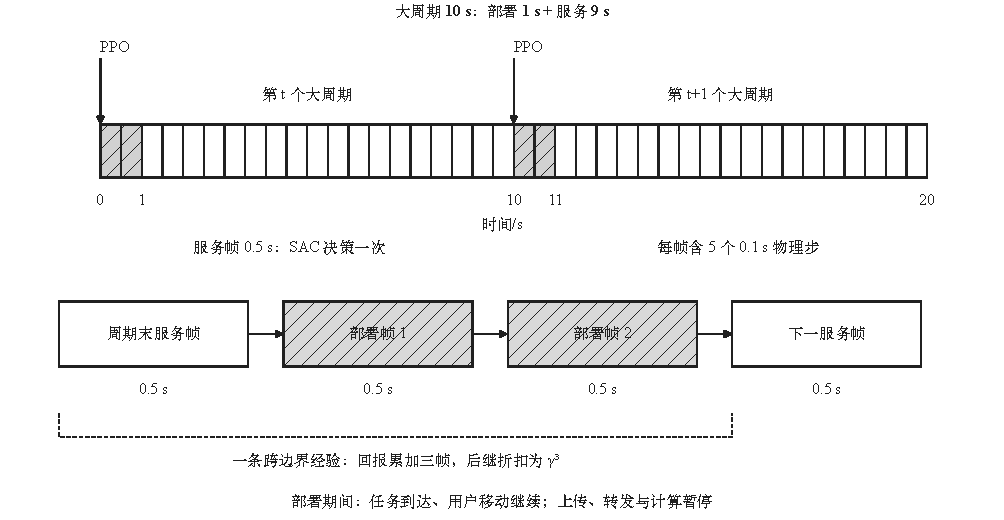
\includegraphics[width=\textwidth]{figures/fig3_timescale.pdf}
\caption{双时间尺度执行时序与跨部署边界经验；顶部时间轴按实际时长绘制}
\label{fig:timescale}
\end{figure*}

令$r_s$为第$s$个资源帧的物理回报，负号将代价最小化转为回报最大化：
\begin{equation}
 r_s=-\sum_{f=0}^{F-1}\gamma_\delta^f c[sF+f].
 \label{eq:framereward}
\end{equation}
此处$f$为帧内物理步索引，与带节点下标的CPU频率$f_{n,p}$按上下文区分。部署帧虽然不进行路由决策，仍然具有由未完成任务和能量账本产生的$r_s$。大层周期回报为
\begin{equation}
 R_t^{\mathrm L}=\frac{1}{J}\sum_{j=0}^{J-1}\gamma^j r_{tJ+j}.
 \label{eq:macroreward}
\end{equation}
式中$j$仅在该求和内表示周期内资源帧索引，$1/J$为常数尺度调整。各周期长度固定时，此调整不改变大层纯回报目标的策略排序。两层没有分别引入“鼓励全部本地”和“鼓励尽量转发”等相互竞争的奖励。

普通服务帧结束后，下一服务帧紧接发生，经验后继折扣为$\gamma$。周期末服务帧结束后，需先经历下一周期的两个部署帧才能再次获得小层决策机会。令$s^\star$为周期末服务帧编号，其跨边界回报和后继折扣为
\begin{equation}
 \widehat r_{s^\star}
 =r_{s^\star}+\gamma r_{s^\star+1}
 +\gamma^2r_{s^\star+2},
 \qquad
 \widehat\gamma_{s^\star}=\gamma^3.
 \label{eq:boundary}
\end{equation}
后继观测取部署结束、下一服务帧当前到达已产生之后的真实观测。上层在边界的部署动作会参与这一转移，不允许把两个部署帧跳过，也不允许用重置后的空队列观测替代真实后继。这使小层转移具有1帧或3帧的不同持时，应按半马尔可夫的持时形式构造目标，而非对所有经验强行使用相同一步折扣。

将普通服务帧的$\widehat r_s$定义为$r_s$、$\widehat\gamma_s$定义为$\gamma$，两类经验可统一记为$(\vct o_s^{\mathrm S},\vct z_s,\vct\rho[s],\widehat r_s,\vct o_{s'}^{\mathrm S},\widehat\gamma_s)$。其中，$s'$是下一次真正的小层决策时刻，不必等于$s+1$。大层经验则使用周期起点及下一周期起点的观测、原始部署动作、周期回报和$\Gamma_{\mathrm L}$。两层观测不同，但读取同一个任务系统；小层处理后的积压自然进入下一次部署观测。

训练中300 s只是统计窗口，不是任务终止时刻。连续采样流覆盖三个窗口，300 s和600 s处均不清空队列。900 s处作为采样截断时，在环境重置之前执行真实下一次部署，并取得下一服务决策观测以补全最后一条小层经验；这些额外步骤不混入此前900 s的性能统计。大层保留真实后继价值，但停止跨重置边界递推优势。固定下层策略时，可研究其诱导的大层转移；联训时下层参数持续变化，大层转移亦随之变化，因此采用两层异频更新不等于获得了两个独立平稳MDP。
